\section{Sprendimo medžių apžvalga}
\label{sec:Sprendimo medziu apzvalga}

\subsection{Bendrieji sprendimo medžių principai}

Sprendimo medžiu vadinamas medžio pavidalo klasifikatorius, priskiriantis klasėms daugiamačius vektorius, kurių požymiai gali būti tiek kategoriniai, tiek tolydieji kintamieji. %[TODO: savybės: privalumai, trūkumai]

Medį sudaro arba lapas, pažymėtas klasės etikete, arba struktūra, apimanti su dviem ar daugiau pomedžių sujungtą sprendimo priėmimo mazgą \cite{DBLP:dblp_journals/csur/Quinlan96}. Pastarosios rūšies mazgai apibrėžiami testo pavidalu, o jų pomedžiai atitinka visas įmanomas šio testo baigtis (pvz., žr. \ref{fig:DT}).
\begin{figure}[H]
  \centering
    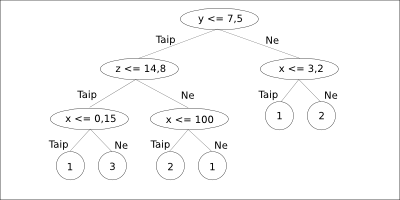
\includegraphics{skyriai/paveiksliukai/sm_pvz}
  \caption{Sprendimo medžio pavyzdys\label{fig:DT}}
\end{figure}

...
